\begin{multicols}{3}[\section{DECT - Digital Enhanced Cordless Telecommunications}]

\rhead{Autor: Simon Retzmann}
\lfoot{Letzte Bearbeitung: 14.04.2016}

\newrefsegment

\begin{boxedminipage}{\linewidth}
\begin{tabular}{p{2,1 cm}p{2.7 cm}}
\textbf{Steckbrief}& \\
\end{tabular}
\begin{tabular}{p{2,1 cm}|p{2.7 cm}}
      Einsatz seit & 1994\\
      \hline
      Frequenz"-bereich  & \SI{1880}-\SI{1900}{\mega\hertz} (Europa)\\
      \hline
      Verbreitung & Weltweit\\
      \hline
      Übertragung & 24 kBit/s pro Kanal (24 Kanäle), jedoch maximal 552 kBit/s, üblicherweise maximal 128 kBit/s\\
      \hline
      Reichweite & bis zu \SI{500}{\meter}\\
      \hline
      Fakten & \begin{itemize}
			\item abhörsicher
			\item hohe Reichweite
			\item geringer Stromverbrauch
		\end{itemize}
				\\
\end{tabular}
\end{boxedminipage}
\par
\subsection*{Überblick}
Der Standard DECT (Digital Enhanced Cordless Telecommunications) ist eine universelle Kurzstrecken-Funktechnik für die Telekommunikation. Im Bereich der schnurlosen Sprachübertragung hat sich DECT weltweit etabliert.
Für eine reibungslose Interaktion mit verschiedenen Telefonnetzen nutzt DECT definierte Zugriffsprotokolle und sogenannten Access Profiles, dadurch kann zum Beispiel eine ISDN oder GSM Konnektivität hergestellt werden. 
Mithilfe der Protokollstruktur können verschiedene Basisstationen zu einem Telefonnetz zusammengeschaltet werden. Unterstützt werden Ein- und Mehrzellensysteme mit gleitendem Übergang zwischen den Zellen, wodurch sich ein DECT-Netz über zum Beispiel größere Firmengelände aufbauen lässt.
\cite{dect.1}
\subsection*{Historische Entwicklung}
Ursprünglich kommt DECT aus Europa und stand für Digital European Cordless Telephone. DECT ist eine Marke vom  European Telecommunications Standards Institute (ETSI) \cite{dect.4}.
\\DECT ist dabei ein weltweit genutzer Standard für Telefonie, doch seit der ersten Veröffentlichung im Jahre 1994 in die Jahre gekommen. In den Zeiten von VoIP hat DECT starke Konkurrenz durch WLAN (IEEE 802.11) bekommen. DECT ist für Sprachübertragung und nicht für Datenübertragung ausgelegt, deswegen haben sich einige Hersteller mit der ETSI zusammengetan und einen neuen Standard erarbeitet. Das Ziel war DECT VoIP- und Datenfähig zu machen, CAT-iq ist dabei herausgekommen. Auf die Weiterentwicklung CAT-iq wird im Laufe des Artikels noch detaillierter eingegangen.
\subsection*{Technische Erläuterungen}
\subsubsection*{Eigenschaften}
In einer internationalen Übereinkunft wurde von der ETSI im DECT Standard festgelegt, dass DECT abhör- und ausfallsicher ist. Außerdem soll nur ein geringes Frequenzband genutzt werden wodurch Frequenzen eingespart werden. Des weiteren soll DECT universell einsetzbar sein mit einer hohen Qualität in der Sprachübertragung. Ein nahtloser Übergang zwischen den Funkzellen ist dabei zu gewährleisten, damit wie bereits erwähnt ein DECT-Netz für ein großes Firmengelände aufgebaut werden kann.

DECT bietet außerdem:
\begin{itemize}
	\item exklusives Frequenzband für den Betrieb
	\item Optimierung auf gleichbleibende Verbindungsqualität und minimaler Verzögerung
	\item hohe Reichweite
	\item geringer Stromverbrauch
	\item geringe Kosten für Endgeräte
	\item Telefonie-Leistungsmerkmale
	\begin{itemize}
		\item gleichzeitiger Betrieb mehrerer Mobilteile
		\item gebührenfreie interne Gespräche
		\item Mobilteile sind an mehreren Basisstationen nutzbar
		\item herstellerunabhängige Nutzung von Mobilteilen an verschiedenen Basisstationen
		\item Handover (automatischer Wechsel der Basisstation)
	\end{itemize}
\end{itemize}
\cite{dect.1}

\subsubsection*{Fixed Part und Portable Part}
Bei DECT ist der Fachbegriff für die  Basisstation der Fixed Part, dieser wechselt seinen Standort nicht. Portable Part ist das Handgerät, also das eigentliche schnurlose Telefon des DECT-Systems. 

Der Fixed Part übernimmt die Vermittlung der Gespräche und stellt dem Benutzer über das Portable Part die Leistungsmerkmale und die Schnittstelle in das leitungsvermittelte Telefonnetz zur Verfügung \cite{dect.1}.


\subsubsection*{Strahlung der DECT-Telefone}
Die schnurlosen Telefone haben einen Eco-Modus, der das Telefon autmatisch in einen Betriebsmodus mit geringen elektromagnetischen Feldern versetzt. Dies wurde aufgrund von Kundennachfragen in fast allen DECT-Telefonen implementiert, denn nach wissenschaftlicher Erkenntnis geht von DECT keine Gefahr aus.

Im Eco-Modus sendet der Fixed Part (die Basistation) mit der Leistung, die notwendig ist, um das am weitesten entfernte Mobilteil zu erreichen. Das bedeutet je näher sich der Portable Part am Fixed Part befindet, desto geringer ist die Funkleistung. Bei einem Portable Part bedeutet es, dass die Funkleistung verringert wird bei Annäherung an den Fixed Part. Bei mehreren Portable Parts müssen alle Geräte sich dem Fixed Part nähern um diesen Effekt zu erreichen. \cite{dect.1}

\subsubsection*{Übertragung}
Für die Übertragung bei DECT wird das Modulationsverfahren GFSK (Gausian Frequency Shift Keying) eingesetzt, da hier effiziente Verstärker genutzt werden können zur Reduktion des Stromverbrauchs und der Wärmeentwicklung.
Die Portable Parts überprüfen ständig die Träger zwischen \SI{1880}-\SI{1900}{\mega\hertz} (10 HF-Kanäle mit \SI{1728}{\kilo\hertz} Abstand). Verwendet wird der Träger mit dem besten Empfangsergebnis. Dieses Verfahren wird Dynamic Channel Selection/Allocation genannt, welches die Störanfälligkeit der Übertragung senkt und gleichzeitig die Sprachqualität erhöht \cite{dect.1}.

\begin{Figure}
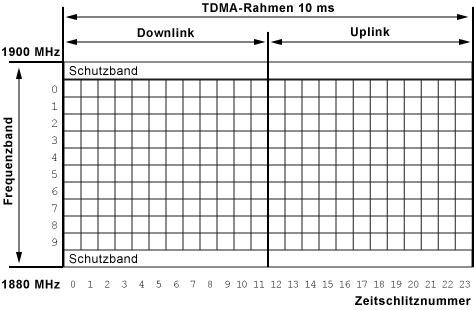
\includegraphics[width=\linewidth]{Kapitel/DECT/Grafiken/frequenzband.png}
\captionof{figure}{Frequenzband von DECT \cite{dect.1}}
\label{fig:dect.frequenzband}
\end{Figure}
Für die Modulation wird das Frequenzband in 10 Frequenzträger unterteilt, jeweils oben und unten befindet sich ein Schutzband, um Störungen durch Überlappungen von anderen Frequenzen zu reduzieren. 

Jeder Frequenzträger wird in 24 Zeitschlitze unterteilt, jeweils 12 Zeitschlitze sind für die Verbindung vom Fixed Part zum Portable Part und umgekehrt reserviert. Die Dauer eines Frames(24 Zeitschlitze) sind 10ms.
Das Nutzsignal wird mit der GFSK Modulation übertragen und bietet eine Bandbreite von 32 kBit/s und bietet damit eine dem Festnetz ähnliche Sprachqualität.

Für die Sprachübertragung werden die Zeitschlitze symmetrisch aufgeteilt, bei Datenübertragungen asymmetrisch mit Bündelung mehrere Kanäle. Bis zu 23 Kanäle lassen sich bündeln, denn es muss nur mindestens ein Kanal für die andere Richtung zur Verfügung stehen \cite{dect.1}.
Die Frequenzmodulation kann allerdings auch mit 4PSK, 8PSK, 16QAM und 64QAM realisiert werden

\subsubsection*{DECT ULE (Ultra-low Energy)}
Bei DECT Ultra-low Energy geht es um die Senkung des Energieverbrauches, die Teilnehmer werden dabei in einen zyklischen Tiefschlaf versetzt. Durch ein Ereignis können die Teilnehmer aus dem Tiefschlaf geholt werden. Kurze Tiefschlafphasen erhöhen allerdings nicht signifikant die Akkulaufzeit, daher wählt man die Pausen möglichst lange, jedoch nicht länger als 20 Sekunden \cite{dect.1}.

\subsubsection*{Datenübertragungen mit DECT}
DECT wurde für die schnurlose Sprachübertragung entwickelt, entsprechend ist DECT zur Datenübertragung nur mit Einschränkungen nutzbar. Mit 24 kBit/s können pro Kanal die Daten übertragen werden. 23 Kanäle lassen sich bündeln, sodass eine Übertragung von 552 kBit/s erreicht werden kann. Üblicherweise können DECT-Datenübertragungsgeräte nur 128 kBit/s übertragen. Mithilfe des DMAP (DECT Multimedia Access Profile) können die vorhandenen 552 kBit/s voll ausgenutzt werden und für ein schurloses Netzwerk auf Basis von DECT verwendet werden. Für die breitbandige Datenübertragung ist dies allerdings nicht ausreichend, weshalb der Nachfolge-Standard CAT-iq entwickelt wurde. \cite{dect.1}

\subsubsection*{GAP - Generic Access Profile}
Das bekannteste DECT-Zugriffsprofil ist das GAP, welches bereits 1994 von ETSI spezifiziert wurde. GAP ermöglicht die Zusammenarbeit zwischen DECT-Geräten unterschiedlicher Hersteller. Alle GAP-kompatiblen Portable Parts lassen sich herstellerunabhängig mit den Telefon-Grundfunktionen an allen GAP-kompatiblen Fixed Parts betreiben. GAP garantiert zwar die Kompatibilität der Mobilteile, jedoch bezieht sich das nur auf die reine Telefonie. Funktionen wie der Anrufbeantworter oder das Telefonbuch funktionieren gegebenenfalls nicht. \cite{dect.4,dect.1}

\subsubsection*{IAP - ISDN Access Networking Profile}
Mithilfe dieser Spezifikation ist ein DECT-Telefon in der Lage ISDN-Komfortmerkmale aus dem Telefonie-Bereich zu nutzen. Zum Beispiel gehört die Rufnummernanzeige, Anklopfen, Dreierkonferenz oder Rufumleitung dazu. Dieses Profil ist weit verbreitet und fast alle DECT-Telefone beherrschen dieses Profil. \cite{dect.1}

\subsubsection*{GIP - GSM Interworking Profile}
Dieses Zugriffsprotokoll regelt die Zusammenarbeit mit digitalen Mobilfunknetzen, die dem GSM-Standard entsprechen (für UMTS existiert auch ein Profil). Mithilfe von Dualmode-Handys lässt sich eine Kombination aus Mobilfunknetz und Festnetz erstellen. Dadurch lässt sich zuhause das Festnetz nutzen und unterwegs das Mobilfunknetz. Unterstützt der Netzbetreiber (Mobilfunk und Festnetz) entsprechende Routing-Techniken, kann für beide Netze dieselbe Telefonnummer angeboten werden. Geräte mit dieser Funktionalität sind jedoch nicht weit verbreitet. \cite{dect.1}
\subsubsection*{DECT CAT-iq}
DECT CAT-iq (Cordless Advanced Technology - internet and quality) soll die Konvergenz von Sprach- und Breitbandübertragungen erhöhen. Neben der Sprachübertragung in Hifi-Qualität können auch Internet-Dienste eingebunden werden. Mithilfe von CAT-iq wird das DECT-Gerät IP-fähig.

Ermöglicht wird damit unter anderem:
\begin{itemize}
\item Musik-Streaming
\item Informationsanzeigen und -dienste aus dem Internet
\item Instant-Messaging 
\item Home-Management-Funktionen
\end{itemize}

Eine Weiterentwicklung von DECT für Datenübertragungen wirkt auf den ersten Blick erst einmal überflüssig. Es stellt sich die Frage warum sollte  etwas neu entwickelt werden, wenn doch die WLAN-Funktechnik genutzt werden könnte zur Übertragung der Daten. Allerdings war WLAN lange nicht als Schnurlostechnik für Telefone geeignet, denn die für die Datenkommunikation ausgelegte WLAN-Technik verbrauchte sehr viel Rechenleistung und hat einen entsprechenden Energieverbrauch. Außerdem funkt WLAN im freien ISM-Band, wo sich auch noch andere Funkanwendungen befinden, weshalb Störungen nicht ausgeschlossen sind. DECT hat den Vorteil ein eigenes Frequenzspektrum zu haben mit einer höheren Reichweite. CAT-iq nutzt den DECT-Frequenzbereich und ist zum bisherigen etablierten DECT-Standard abwärtskompatibel. \cite{dect.3}
\subsection*{Einsatz}
DECT ist als ETSI-Standard für  Kurzstrecken-Funktechnik entwickelt worden und kann für viele Anwendungen in der ganzen Welt in unlizensierten Frequenzbereichen genutzt werden. DECT ist für Telefonie (PSTN und VoIP) und Datenübertragung entwickelt mit einer Reichweite bis zu 500 Metern.

Seit Beginn wurden mehr als 820 Millionen Geräte hergestellt, jährlich kommen ca. 100 Millionen Geräte dazu. DECT dominiert den kabellosen Sprachübertragungssektor mit einem Marktanteil von 73\% von allen kabellosen Technologien (inklusive analogen und proprietären). DECT erhält mehr Marktanteil durch den Austausch von alten analogen Technologien, aber wird verliert auch Marktanteile durch die digitalen Technologien basierend auf IEEE 802.11. Die geringen Kosten von DECT Chipsätzen durch die Massenproduktion erlauben den Austausch von fest verkabelten Telefonen.

DECT wurde initial für Europa entwickelt, ist jedoch mittlerweile in über 110 Ländern adoptiert worden. Die Vereinigten Staaten von Amerika haben sich gegenüber DECT über eine FCC Entscheidung 2005 geöffnet und sind mit der wichtigste Markt hinsichtlich des Wachstums. Japan hat sich vor kurzem auch DECT geöffnet, wo noch traditionell der Markt von The Personal Handy-phone System (PHS) dominiert wird.

Seit 2010 haben viele Betreiber in Europa ihre Telefonnetze auf IP-Netze umgestellt, damit geht eine qualitative Verbesserung der Sprachqualität einher. Statt bisher \SI{3.1}{\kilo\hertz} soll mindestens das Doppelte zur Verfügung stehen. Viele Endgeräte unterstützen  diesen sogenannten HD-Sound bereits.


Neuerungen:
Parallel zur Telefonie können noch weitere Daten übertragen werden, wie z.B. ein externes Adressbuch, Webradio oder ähnliches.
\cite{dect.3,dect.5}
\subsection*{Ausblick}
Innerhalb von Europa sind folgende Frequenzen für DECT reserviert:
\begin{itemize}
\item \SI{1900}-\SI{1920}{\mega\hertz} (geteilt mit UTRAN TDD)
\item \SI{1920}-\SI{1980}{\mega\hertz} (geteilt mit dem Uplink von UTRAN FDD)
\item \SI{2010}-\SI{2025}{\mega\hertz} (vorgesehen für die potentielle Erweiterung von IMT-2000, noch nicht genutzt)
\end{itemize} 

\subsubsection*{Konkurrenz Voice-over-WLAN (VoWLAN)}
WLAN wurde nicht für die Sprachübertragung ausgelegt, jedoch wird mit dem Standard IEEE 802.11e Voice-over-WLAN die Sprachübertragung ermöglicht.

DECT ist für Sprachkommunikation ausgelegt und dank des modularen Aufbaus lassen sich DECT-Netze bei Bedarf mit weiteren Basisstationen erweitern. Durch nahtloses Handover wird eine ständige Konnektivität gewährleistet.

Bei VoWLAN existiert gerade bei Unternehmen in der Regel bereits eine Infrastruktur, weshalb Kosten gespart werden können, da nicht ein weiteres Funknetz aufgebaut werden muss. Allerdings haben DECT Geräte eine längere Akkulaufzeit durch einen geringeren Energieverbrauch als VoWLAN-Geräte.
Letztendlich hängt die Entscheidung zwischen DECT und VoWLAN vor allem von der bestehenden Infrastruktur ab. Wird diese allerdings neu aufgebaut, dann ist es in der Regel günstiger VoWLAN zu nutzen, da keine zwei Infrastrukturen aufgebaut werden müssen. Diese Kostenersparnis wird für viele relevant sein, weshalb DECT eventuell in Zukunft vom Markt verschwinden könnte. WLAN entwickelt sich damit immer mehr zu einer universellen Standard-Infrastruktur. 

Für den Heimanwendungsbereich bietet zum Beispiel die FritzBox in den neueren Modellen mehrere Möglichkeiten. Der DECT Standard ist implementiert, jedoch wird auch eine App für Smartphones zur Verfügung gestellt, mit der man mit seinem Smartphone über WLAN telefonieren kann. 
\cite{dect.6,dect.7,dect.8}
\printbibliography[segment=1,heading=subbibliography]
\end{multicols}

\newpage
